\documentclass[twoside]{book}

% Packages required by doxygen
\usepackage{calc}
\usepackage{doxygen}
\usepackage{graphicx}
\usepackage[utf8]{inputenc}
\usepackage{makeidx}
\usepackage{multicol}
\usepackage{multirow}
\usepackage{textcomp}
\usepackage[table]{xcolor}

% Font selection
\usepackage[T1]{fontenc}
\usepackage{mathptmx}
\usepackage[scaled=.90]{helvet}
\usepackage{courier}
\usepackage{amssymb}
\usepackage{sectsty}
\renewcommand{\familydefault}{\sfdefault}
\allsectionsfont{%
  \fontseries{bc}\selectfont%
  \color{darkgray}%
}
\renewcommand{\DoxyLabelFont}{%
  \fontseries{bc}\selectfont%
  \color{darkgray}%
}

% Page & text layout
\usepackage{geometry}
\geometry{%
  a4paper,%
  top=2.5cm,%
  bottom=2.5cm,%
  left=2.5cm,%
  right=2.5cm%
}
\tolerance=750
\hfuzz=15pt
\hbadness=750
\setlength{\emergencystretch}{15pt}
\setlength{\parindent}{0cm}
\setlength{\parskip}{0.2cm}
\makeatletter
\renewcommand{\paragraph}{%
  \@startsection{paragraph}{4}{0ex}{-1.0ex}{1.0ex}{%
    \normalfont\normalsize\bfseries\SS@parafont%
  }%
}
\renewcommand{\subparagraph}{%
  \@startsection{subparagraph}{5}{0ex}{-1.0ex}{1.0ex}{%
    \normalfont\normalsize\bfseries\SS@subparafont%
  }%
}
\makeatother

% Headers & footers
\usepackage{fancyhdr}
\pagestyle{fancyplain}
\fancyhead[LE]{\fancyplain{}{\bfseries\thepage}}
\fancyhead[CE]{\fancyplain{}{}}
\fancyhead[RE]{\fancyplain{}{\bfseries\leftmark}}
\fancyhead[LO]{\fancyplain{}{\bfseries\rightmark}}
\fancyhead[CO]{\fancyplain{}{}}
\fancyhead[RO]{\fancyplain{}{\bfseries\thepage}}
\fancyfoot[LE]{\fancyplain{}{}}
\fancyfoot[CE]{\fancyplain{}{}}
\fancyfoot[RE]{\fancyplain{}{\bfseries\scriptsize Generated on Wed Mar 11 2015 11\-:57\-:06 for Ntuple Code by Doxygen }}
\fancyfoot[LO]{\fancyplain{}{\bfseries\scriptsize Generated on Wed Mar 11 2015 11\-:57\-:06 for Ntuple Code by Doxygen }}
\fancyfoot[CO]{\fancyplain{}{}}
\fancyfoot[RO]{\fancyplain{}{}}
\renewcommand{\footrulewidth}{0.4pt}
\renewcommand{\chaptermark}[1]{%
  \markboth{#1}{}%
}
\renewcommand{\sectionmark}[1]{%
  \markright{\thesection\ #1}%
}

% Indices & bibliography
\usepackage{natbib}
\usepackage[titles]{tocloft}
\setcounter{tocdepth}{3}
\setcounter{secnumdepth}{5}
\makeindex

% Hyperlinks (required, but should be loaded last)
\usepackage{ifpdf}
\ifpdf
  \usepackage[pdftex,pagebackref=true]{hyperref}
\else
  \usepackage[ps2pdf,pagebackref=true]{hyperref}
\fi
\hypersetup{%
  colorlinks=true,%
  linkcolor=blue,%
  citecolor=blue,%
  unicode%
}

% Custom commands
\newcommand{\clearemptydoublepage}{%
  \newpage{\pagestyle{empty}\cleardoublepage}%
}


%===== C O N T E N T S =====

\begin{document}

% Titlepage & ToC
\hypersetup{pageanchor=false}
\pagenumbering{roman}
\begin{titlepage}
\vspace*{7cm}
\begin{center}%
{\Large Ntuple Code }\\
\vspace*{1cm}
{\large Generated by Doxygen 1.8.5}\\
\vspace*{0.5cm}
{\small Wed Mar 11 2015 11:57:06}\\
\end{center}
\end{titlepage}
\clearemptydoublepage
\tableofcontents
\clearemptydoublepage
\pagenumbering{arabic}
\hypersetup{pageanchor=true}

%--- Begin generated contents ---
\chapter{Namespace Index}
\section{Namespace List}
Here is a list of all documented namespaces with brief descriptions\-:\begin{DoxyCompactList}
\item\contentsline{section}{\hyperlink{namespaceran}{ran} \\*R\-A\-L Analysis Ntuples library namespace }{\pageref{namespaceran}}{}
\end{DoxyCompactList}

\chapter{Hierarchical Index}
\section{Class Hierarchy}
This inheritance list is sorted roughly, but not completely, alphabetically\-:\begin{DoxyCompactList}
\item E\-D\-Analyzer\begin{DoxyCompactList}
\item \contentsline{section}{Mini\-Analyzer}{\pageref{classMiniAnalyzer}}{}
\end{DoxyCompactList}
\item \contentsline{section}{ran\-:\-:Nt\-Electron}{\pageref{classran_1_1NtElectron}}{}
\item \contentsline{section}{ran\-:\-:Nt\-Jet}{\pageref{classran_1_1NtJet}}{}
\item \contentsline{section}{ran\-:\-:Nt\-Muon}{\pageref{classran_1_1NtMuon}}{}
\item \contentsline{section}{Ntp\-Reader}{\pageref{classNtpReader}}{}
\item T\-Object\begin{DoxyCompactList}
\item \contentsline{section}{ran\-:\-:Electron\-Struct}{\pageref{classran_1_1ElectronStruct}}{}
\item \contentsline{section}{ran\-:\-:Event\-Info}{\pageref{classran_1_1EventInfo}}{}
\item \contentsline{section}{ran\-:\-:Jet\-Struct}{\pageref{structran_1_1JetStruct}}{}
\item \contentsline{section}{ran\-:\-:Muon\-Struct}{\pageref{structran_1_1MuonStruct}}{}
\end{DoxyCompactList}
\end{DoxyCompactList}

\chapter{Class Index}
\section{Class List}
Here are the classes, structs, unions and interfaces with brief descriptions\-:\begin{DoxyCompactList}
\item\contentsline{section}{\hyperlink{classran_1_1ElectronStruct}{ran\-::\-Electron\-Struct} }{\pageref{classran_1_1ElectronStruct}}{}
\item\contentsline{section}{\hyperlink{classran_1_1EventInfo}{ran\-::\-Event\-Info} }{\pageref{classran_1_1EventInfo}}{}
\item\contentsline{section}{\hyperlink{structran_1_1JetStruct}{ran\-::\-Jet\-Struct} }{\pageref{structran_1_1JetStruct}}{}
\item\contentsline{section}{\hyperlink{classMiniAnalyzer}{Mini\-Analyzer} }{\pageref{classMiniAnalyzer}}{}
\item\contentsline{section}{\hyperlink{structran_1_1MuonStruct}{ran\-::\-Muon\-Struct} }{\pageref{structran_1_1MuonStruct}}{}
\item\contentsline{section}{\hyperlink{classran_1_1NtElectron}{ran\-::\-Nt\-Electron} }{\pageref{classran_1_1NtElectron}}{}
\item\contentsline{section}{\hyperlink{classran_1_1NtJet}{ran\-::\-Nt\-Jet} }{\pageref{classran_1_1NtJet}}{}
\item\contentsline{section}{\hyperlink{classran_1_1NtMuon}{ran\-::\-Nt\-Muon} }{\pageref{classran_1_1NtMuon}}{}
\item\contentsline{section}{\hyperlink{classNtpReader}{Ntp\-Reader} }{\pageref{classNtpReader}}{}
\end{DoxyCompactList}

\chapter{Namespace Documentation}
\hypertarget{namespaceran}{\section{ran Namespace Reference}
\label{namespaceran}\index{ran@{ran}}
}


R\-A\-L Analysis Ntuples library namespace.  


\subsection*{Classes}
\begin{DoxyCompactItemize}
\item 
class \hyperlink{classran_1_1ElectronStruct}{Electron\-Struct}
\item 
class \hyperlink{classran_1_1EventInfo}{Event\-Info}
\item 
struct \hyperlink{structran_1_1JetStruct}{Jet\-Struct}
\item 
struct \hyperlink{structran_1_1MuonStruct}{Muon\-Struct}
\item 
class \hyperlink{classran_1_1NtElectron}{Nt\-Electron}
\item 
class \hyperlink{classran_1_1NtJet}{Nt\-Jet}
\item 
class \hyperlink{classran_1_1NtMuon}{Nt\-Muon}
\end{DoxyCompactItemize}


\subsection{Detailed Description}
R\-A\-L Analysis Ntuples library namespace. 
\chapter{Class Documentation}
\hypertarget{classran_1_1ElectronStruct}{\section{ran\-:\-:Electron\-Struct Class Reference}
\label{classran_1_1ElectronStruct}\index{ran\-::\-Electron\-Struct@{ran\-::\-Electron\-Struct}}
}
Inheritance diagram for ran\-:\-:Electron\-Struct\-:\begin{figure}[H]
\begin{center}
\leavevmode
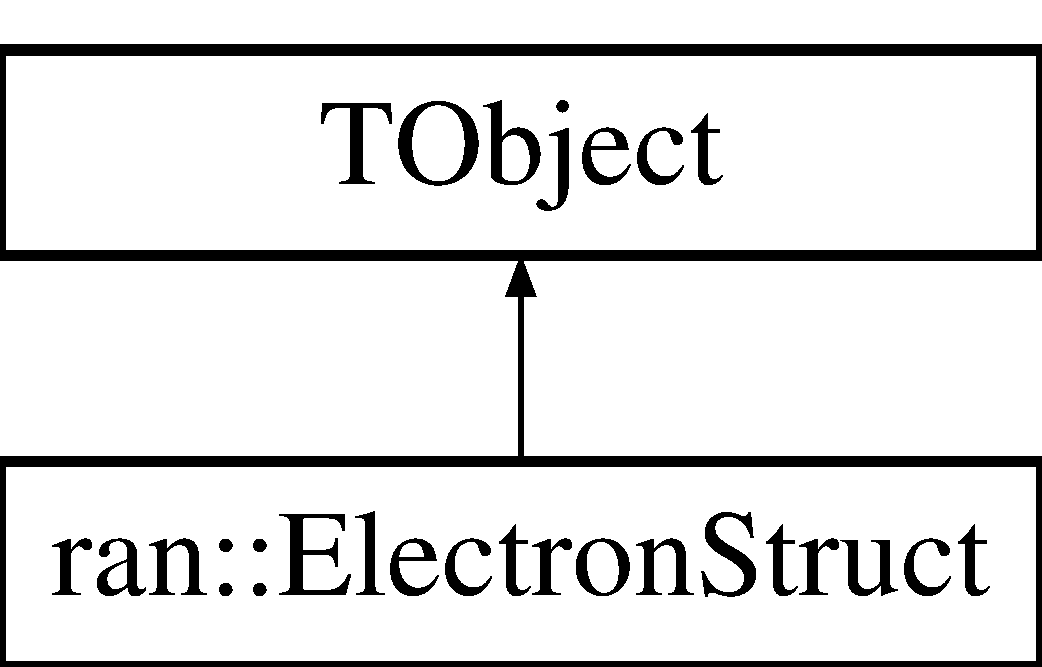
\includegraphics[height=2.000000cm]{classran_1_1ElectronStruct}
\end{center}
\end{figure}
\subsection*{Public Member Functions}
\begin{DoxyCompactItemize}
\item 
\hypertarget{classran_1_1ElectronStruct_afb7806d66cffdb8eeab1b0a7f64fa7f1}{\hyperlink{classran_1_1ElectronStruct_afb7806d66cffdb8eeab1b0a7f64fa7f1}{Electron\-Struct} ()}\label{classran_1_1ElectronStruct_afb7806d66cffdb8eeab1b0a7f64fa7f1}

\begin{DoxyCompactList}\small\item\em default constructor \end{DoxyCompactList}\item 
\hypertarget{classran_1_1ElectronStruct_a53b22b327ab22c53754017765e92fc1a}{virtual \hyperlink{classran_1_1ElectronStruct_a53b22b327ab22c53754017765e92fc1a}{$\sim$\-Electron\-Struct} ()}\label{classran_1_1ElectronStruct_a53b22b327ab22c53754017765e92fc1a}

\begin{DoxyCompactList}\small\item\em virtual destructor \end{DoxyCompactList}\end{DoxyCompactItemize}
\subsection*{Public Attributes}
\begin{DoxyCompactItemize}
\item 
\hypertarget{classran_1_1ElectronStruct_a0533ebb8b7ad7c5baad0b2cb98c72930}{double \hyperlink{classran_1_1ElectronStruct_a0533ebb8b7ad7c5baad0b2cb98c72930}{pt}}\label{classran_1_1ElectronStruct_a0533ebb8b7ad7c5baad0b2cb98c72930}

\begin{DoxyCompactList}\small\item\em electron pt \end{DoxyCompactList}\item 
\hypertarget{classran_1_1ElectronStruct_a155d30dfe051067d4266683dd591ab86}{double \hyperlink{classran_1_1ElectronStruct_a155d30dfe051067d4266683dd591ab86}{eta}}\label{classran_1_1ElectronStruct_a155d30dfe051067d4266683dd591ab86}

\begin{DoxyCompactList}\small\item\em electron eta \end{DoxyCompactList}\item 
\hypertarget{classran_1_1ElectronStruct_ae521033100c5ea87dd7027bf7b34b609}{bool \hyperlink{classran_1_1ElectronStruct_ae521033100c5ea87dd7027bf7b34b609}{gsf\-Track\-\_\-available}}\label{classran_1_1ElectronStruct_ae521033100c5ea87dd7027bf7b34b609}

\begin{DoxyCompactList}\small\item\em Is G\-S\-F track available. \end{DoxyCompactList}\item 
\hypertarget{classran_1_1ElectronStruct_a4974e31d5aebf18e0f304a44b63cb0f8}{double \hyperlink{classran_1_1ElectronStruct_a4974e31d5aebf18e0f304a44b63cb0f8}{sc\-Eta}}\label{classran_1_1ElectronStruct_a4974e31d5aebf18e0f304a44b63cb0f8}

\begin{DoxyCompactList}\small\item\em super cluster eta \end{DoxyCompactList}\item 
\hypertarget{classran_1_1ElectronStruct_a81584bef367cf1c6b30e20748cf1d99c}{double \hyperlink{classran_1_1ElectronStruct_a81584bef367cf1c6b30e20748cf1d99c}{sc\-Energy}}\label{classran_1_1ElectronStruct_a81584bef367cf1c6b30e20748cf1d99c}

\begin{DoxyCompactList}\small\item\em super cluster energy \end{DoxyCompactList}\item 
\hypertarget{classran_1_1ElectronStruct_a67aec0172a6f49670ff60621436da58b}{bool \hyperlink{classran_1_1ElectronStruct_a67aec0172a6f49670ff60621436da58b}{ecal\-Driven\-Seed}}\label{classran_1_1ElectronStruct_a67aec0172a6f49670ff60621436da58b}

\begin{DoxyCompactList}\small\item\em is ecal driven \end{DoxyCompactList}\item 
\hypertarget{classran_1_1ElectronStruct_a443b77544f6e958df3143b92cbc7f375}{double \hyperlink{classran_1_1ElectronStruct_a443b77544f6e958df3143b92cbc7f375}{e2x5\-Max}}\label{classran_1_1ElectronStruct_a443b77544f6e958df3143b92cbc7f375}

\begin{DoxyCompactList}\small\item\em e2x5 max \end{DoxyCompactList}\item 
\hypertarget{classran_1_1ElectronStruct_a550e3ae93aa6c792d3a95124098f7d36}{double \hyperlink{classran_1_1ElectronStruct_a550e3ae93aa6c792d3a95124098f7d36}{e5x5}}\label{classran_1_1ElectronStruct_a550e3ae93aa6c792d3a95124098f7d36}

\begin{DoxyCompactList}\small\item\em e5x5 \end{DoxyCompactList}\item 
\hypertarget{classran_1_1ElectronStruct_ad1f8f2b90dfa55301226469dc6b61d62}{double \hyperlink{classran_1_1ElectronStruct_ad1f8f2b90dfa55301226469dc6b61d62}{e1x5}}\label{classran_1_1ElectronStruct_ad1f8f2b90dfa55301226469dc6b61d62}

\begin{DoxyCompactList}\small\item\em e1x5 \end{DoxyCompactList}\item 
\hypertarget{classran_1_1ElectronStruct_a2d2124c3b49a224413876ad06111817e}{double {\bfseries delta\-Phi\-Super\-Cluster\-Track\-At\-Vtx}}\label{classran_1_1ElectronStruct_a2d2124c3b49a224413876ad06111817e}

\item 
\hypertarget{classran_1_1ElectronStruct_aae2e545a08694e0e38d37fc675cd0afd}{double \hyperlink{classran_1_1ElectronStruct_aae2e545a08694e0e38d37fc675cd0afd}{hadronic\-Over\-Em}}\label{classran_1_1ElectronStruct_aae2e545a08694e0e38d37fc675cd0afd}

\begin{DoxyCompactList}\small\item\em H/\-E. \end{DoxyCompactList}\item 
\hypertarget{classran_1_1ElectronStruct_a5c71622e2493756dcc0a395840a25763}{double {\bfseries sc\-Sigma\-I\-Eta\-I\-Eta}}\label{classran_1_1ElectronStruct_a5c71622e2493756dcc0a395840a25763}

\item 
\hypertarget{classran_1_1ElectronStruct_a84a4986795c6fabfafd37387db1c17fc}{double {\bfseries dr03\-Ecal\-Rec\-Hit\-Sum\-Et}}\label{classran_1_1ElectronStruct_a84a4986795c6fabfafd37387db1c17fc}

\item 
\hypertarget{classran_1_1ElectronStruct_aa073696de03fd8e30256b9dc2f4c0d48}{double {\bfseries dr03\-Hcal\-Depth1\-Tower\-Sum\-Et}}\label{classran_1_1ElectronStruct_aa073696de03fd8e30256b9dc2f4c0d48}

\item 
\hypertarget{classran_1_1ElectronStruct_adbd039800bfdaa5b057a55e7e06dc7f3}{double {\bfseries dr03\-Tk\-Sum\-Pt}}\label{classran_1_1ElectronStruct_adbd039800bfdaa5b057a55e7e06dc7f3}

\item 
\hypertarget{classran_1_1ElectronStruct_a6665fd08e43947dd118fc8c646cf136c}{double \hyperlink{classran_1_1ElectronStruct_a6665fd08e43947dd118fc8c646cf136c}{sigma\-Ieta\-Ieta}}\label{classran_1_1ElectronStruct_a6665fd08e43947dd118fc8c646cf136c}

\begin{DoxyCompactList}\small\item\em sigma\-Ieta\-Ieta \end{DoxyCompactList}\item 
\hypertarget{classran_1_1ElectronStruct_a629f78a9ec38d7d846fdd63411488f7e}{double \hyperlink{classran_1_1ElectronStruct_a629f78a9ec38d7d846fdd63411488f7e}{full5x5\-\_\-sigma\-Ieta\-Ieta}}\label{classran_1_1ElectronStruct_a629f78a9ec38d7d846fdd63411488f7e}

\begin{DoxyCompactList}\small\item\em full5x5\-\_\-sigma\-Ieta\-Ieta \end{DoxyCompactList}\item 
\hypertarget{classran_1_1ElectronStruct_a0155c87ef590c4da51a35595ef3e1945}{bool \hyperlink{classran_1_1ElectronStruct_a0155c87ef590c4da51a35595ef3e1945}{pass\-Conversion\-Veto}}\label{classran_1_1ElectronStruct_a0155c87ef590c4da51a35595ef3e1945}

\begin{DoxyCompactList}\small\item\em pass\-Conversion\-Veto \end{DoxyCompactList}\end{DoxyCompactItemize}


The documentation for this class was generated from the following files\-:\begin{DoxyCompactItemize}
\item 
interface/Electron\-Struct.\-hh\item 
src/Electron\-Struct.\-cc\end{DoxyCompactItemize}

\hypertarget{classran_1_1EventInfo}{\section{ran\-:\-:Event\-Info Class Reference}
\label{classran_1_1EventInfo}\index{ran\-::\-Event\-Info@{ran\-::\-Event\-Info}}
}
Inheritance diagram for ran\-:\-:Event\-Info\-:\begin{figure}[H]
\begin{center}
\leavevmode
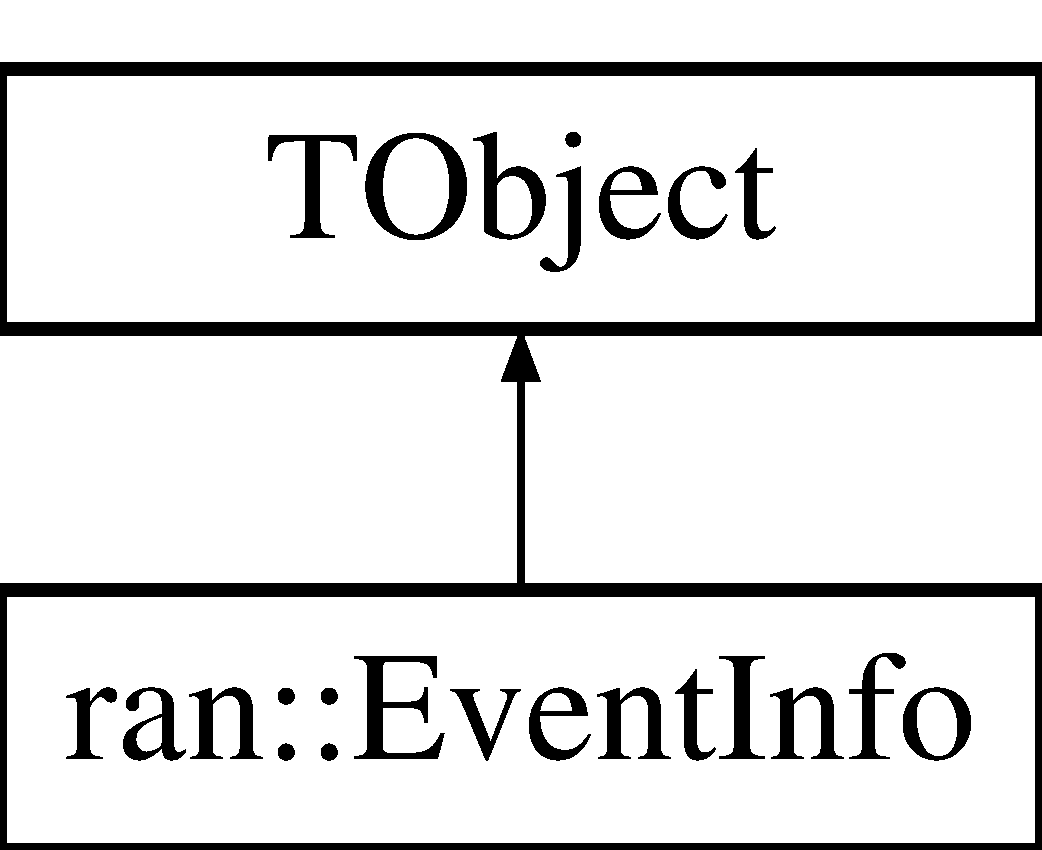
\includegraphics[height=2.000000cm]{classran_1_1EventInfo}
\end{center}
\end{figure}
\subsection*{Public Member Functions}
\begin{DoxyCompactItemize}
\item 
\hypertarget{classran_1_1EventInfo_a1713048bd2b1cd5cc12ec4200ecb668a}{\hyperlink{classran_1_1EventInfo_a1713048bd2b1cd5cc12ec4200ecb668a}{Event\-Info} ()}\label{classran_1_1EventInfo_a1713048bd2b1cd5cc12ec4200ecb668a}

\begin{DoxyCompactList}\small\item\em \hyperlink{classran_1_1EventInfo}{Event\-Info} Constructor. \end{DoxyCompactList}\end{DoxyCompactItemize}
\subsection*{Public Attributes}
\begin{DoxyCompactItemize}
\item 
\hypertarget{classran_1_1EventInfo_a49143c41c768684f24f10d210d727524}{unsigned int \hyperlink{classran_1_1EventInfo_a49143c41c768684f24f10d210d727524}{evt\-Num}}\label{classran_1_1EventInfo_a49143c41c768684f24f10d210d727524}

\begin{DoxyCompactList}\small\item\em Event number. \end{DoxyCompactList}\item 
\hypertarget{classran_1_1EventInfo_ab68aab06dc922ba7044ec3195de5b7d3}{unsigned int \hyperlink{classran_1_1EventInfo_ab68aab06dc922ba7044ec3195de5b7d3}{run\-Num}}\label{classran_1_1EventInfo_ab68aab06dc922ba7044ec3195de5b7d3}

\begin{DoxyCompactList}\small\item\em Run number. \end{DoxyCompactList}\item 
\hypertarget{classran_1_1EventInfo_a76b1e0e67f2b8c1143a6b85ec63ba3a0}{unsigned int \hyperlink{classran_1_1EventInfo_a76b1e0e67f2b8c1143a6b85ec63ba3a0}{lumi\-Sec}}\label{classran_1_1EventInfo_a76b1e0e67f2b8c1143a6b85ec63ba3a0}

\begin{DoxyCompactList}\small\item\em lumisec \end{DoxyCompactList}\end{DoxyCompactItemize}


The documentation for this class was generated from the following files\-:\begin{DoxyCompactItemize}
\item 
interface/Event\-Info.\-hh\item 
src/Event\-Info.\-cc\end{DoxyCompactItemize}

\hypertarget{structran_1_1JetStruct}{\section{ran\-:\-:Jet\-Struct Struct Reference}
\label{structran_1_1JetStruct}\index{ran\-::\-Jet\-Struct@{ran\-::\-Jet\-Struct}}
}
Inheritance diagram for ran\-:\-:Jet\-Struct\-:\begin{figure}[H]
\begin{center}
\leavevmode
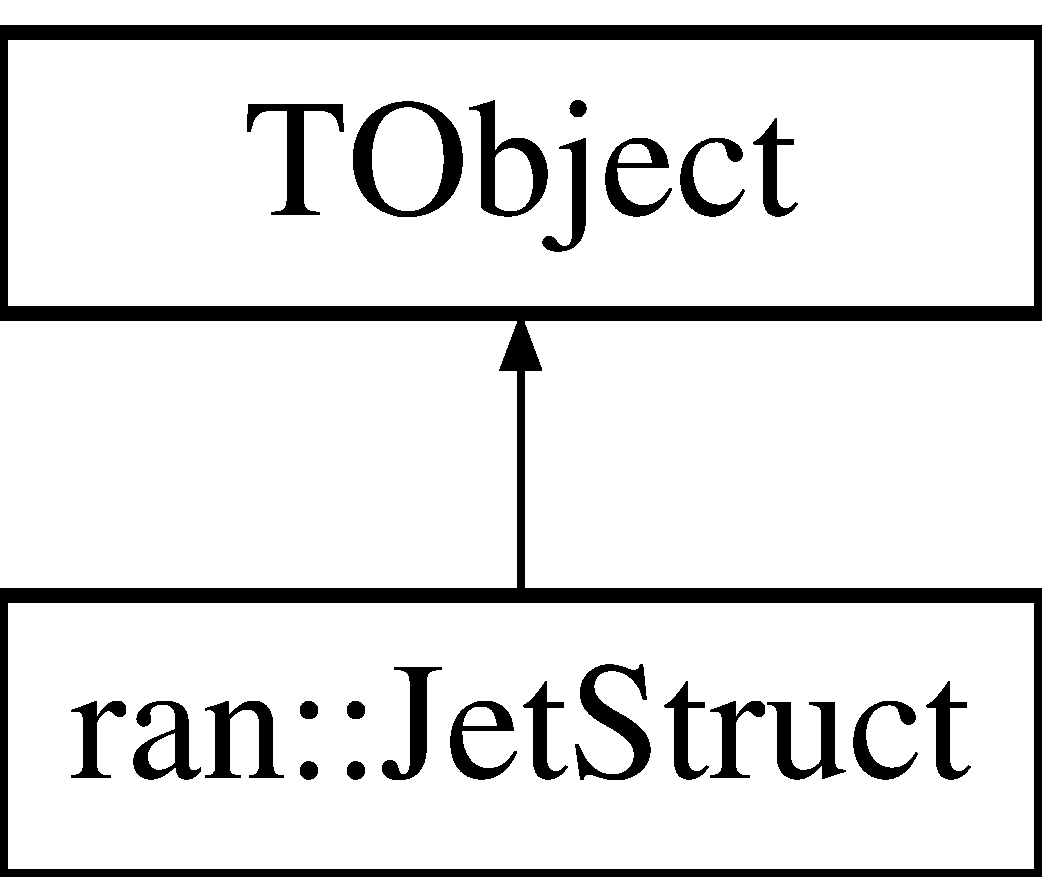
\includegraphics[height=2.000000cm]{structran_1_1JetStruct}
\end{center}
\end{figure}
\subsection*{Public Member Functions}
\begin{DoxyCompactItemize}
\item 
\hypertarget{structran_1_1JetStruct_a080ad77c3499f07562a6409e915beac5}{\hyperlink{structran_1_1JetStruct_a080ad77c3499f07562a6409e915beac5}{Jet\-Struct} ()}\label{structran_1_1JetStruct_a080ad77c3499f07562a6409e915beac5}

\begin{DoxyCompactList}\small\item\em default constructor \end{DoxyCompactList}\item 
\hypertarget{structran_1_1JetStruct_a57e72fe40bf4a2757825da6b8eb703ba}{virtual \hyperlink{structran_1_1JetStruct_a57e72fe40bf4a2757825da6b8eb703ba}{$\sim$\-Jet\-Struct} ()}\label{structran_1_1JetStruct_a57e72fe40bf4a2757825da6b8eb703ba}

\begin{DoxyCompactList}\small\item\em destructor \end{DoxyCompactList}\end{DoxyCompactItemize}
\subsection*{Public Attributes}
\begin{DoxyCompactItemize}
\item 
\hypertarget{structran_1_1JetStruct_a935690381685df633c696534d0ac6216}{double \hyperlink{structran_1_1JetStruct_a935690381685df633c696534d0ac6216}{et}}\label{structran_1_1JetStruct_a935690381685df633c696534d0ac6216}

\begin{DoxyCompactList}\small\item\em et \end{DoxyCompactList}\item 
\hypertarget{structran_1_1JetStruct_abcccf8da31a44023609d0a768eb05221}{double {\bfseries pt}}\label{structran_1_1JetStruct_abcccf8da31a44023609d0a768eb05221}

\item 
\hypertarget{structran_1_1JetStruct_a46830c9571b7065d242d099ae64b4875}{double \hyperlink{structran_1_1JetStruct_a46830c9571b7065d242d099ae64b4875}{mass}}\label{structran_1_1JetStruct_a46830c9571b7065d242d099ae64b4875}

\begin{DoxyCompactList}\small\item\em $<$ pt \end{DoxyCompactList}\item 
double \hyperlink{structran_1_1JetStruct_a164bcdb9e674202cd0e73ee7fabafd36}{eta}
\begin{DoxyCompactList}\small\item\em $<$ mass \end{DoxyCompactList}\item 
\hypertarget{structran_1_1JetStruct_a1291f96fa4663a65c252a510538723d5}{double \hyperlink{structran_1_1JetStruct_a1291f96fa4663a65c252a510538723d5}{jet\-Probability\-B\-Jet\-Tags}}\label{structran_1_1JetStruct_a1291f96fa4663a65c252a510538723d5}

\begin{DoxyCompactList}\small\item\em jet\-Probability\-B\-Jet\-Tags b tag discriminator \end{DoxyCompactList}\item 
\hypertarget{structran_1_1JetStruct_a8da7809055faff45b30b70a43ac67447}{double \hyperlink{structran_1_1JetStruct_a8da7809055faff45b30b70a43ac67447}{jet\-B\-Probability\-B\-Jet\-Tags}}\label{structran_1_1JetStruct_a8da7809055faff45b30b70a43ac67447}

\begin{DoxyCompactList}\small\item\em jet\-B\-Probability\-B\-Jet\-Tags b tag discriminator \end{DoxyCompactList}\item 
\hypertarget{structran_1_1JetStruct_ae56ed74e0854b7ba96bb58aee24e3c37}{double \hyperlink{structran_1_1JetStruct_ae56ed74e0854b7ba96bb58aee24e3c37}{track\-Counting\-High\-Eff\-B\-Jet\-Tags}}\label{structran_1_1JetStruct_ae56ed74e0854b7ba96bb58aee24e3c37}

\begin{DoxyCompactList}\small\item\em track\-Counting\-High\-Eff\-B\-Jet\-Tags b tag discriminator \end{DoxyCompactList}\item 
\hypertarget{structran_1_1JetStruct_ad1c745b77d4cca7b28b2d2df36fec075}{double \hyperlink{structran_1_1JetStruct_ad1c745b77d4cca7b28b2d2df36fec075}{track\-Counting\-High\-Pur\-B\-Jet\-Tags}}\label{structran_1_1JetStruct_ad1c745b77d4cca7b28b2d2df36fec075}

\begin{DoxyCompactList}\small\item\em track\-Counting\-High\-Pur\-B\-Jet\-Tags b tag discriminator \end{DoxyCompactList}\item 
\hypertarget{structran_1_1JetStruct_a96b9bfecc789790ee654d542efbc0d6b}{double \hyperlink{structran_1_1JetStruct_a96b9bfecc789790ee654d542efbc0d6b}{simple\-Secondary\-Vertex\-High\-Eff\-B\-Jet\-Tags}}\label{structran_1_1JetStruct_a96b9bfecc789790ee654d542efbc0d6b}

\begin{DoxyCompactList}\small\item\em simple\-Secondary\-Vertex\-High\-Eff\-B\-Jet\-Tags b tag discriminator \end{DoxyCompactList}\item 
\hypertarget{structran_1_1JetStruct_a76534a95f4373c87ca6b70f8e65965e1}{double \hyperlink{structran_1_1JetStruct_a76534a95f4373c87ca6b70f8e65965e1}{simple\-Secondary\-Vertex\-High\-Pur\-B\-Jet\-Tags}}\label{structran_1_1JetStruct_a76534a95f4373c87ca6b70f8e65965e1}

\begin{DoxyCompactList}\small\item\em combined\-Secondary\-Vertex\-B\-Jet\-Tags b tag discriminator \end{DoxyCompactList}\item 
\hypertarget{structran_1_1JetStruct_a78ad7fb27ed4e35314273a3e7b54fd84}{double \hyperlink{structran_1_1JetStruct_a78ad7fb27ed4e35314273a3e7b54fd84}{combined\-Inclusive\-Secondary\-Vertex\-B\-Jet\-Tags}}\label{structran_1_1JetStruct_a78ad7fb27ed4e35314273a3e7b54fd84}

\begin{DoxyCompactList}\small\item\em combined\-Inclusive\-Secondary\-Vertex\-B\-Jet\-Tags b tag discriminator \end{DoxyCompactList}\item 
\hypertarget{structran_1_1JetStruct_ae50fb1fdad429bab2f944bc355151ca6}{double \hyperlink{structran_1_1JetStruct_ae50fb1fdad429bab2f944bc355151ca6}{jec\-Factor\-\_\-un\-Corrected}}\label{structran_1_1JetStruct_ae50fb1fdad429bab2f944bc355151ca6}

\begin{DoxyCompactList}\small\item\em factor applied to jet pt to get uncorrect jet pt \end{DoxyCompactList}\item 
\hypertarget{structran_1_1JetStruct_a15787ddfba12fd8027ece6a1fec3fd0a}{double \hyperlink{structran_1_1JetStruct_a15787ddfba12fd8027ece6a1fec3fd0a}{user\-Float\-\_\-pileup\-Jet\-Id\-\_\-full\-Discriminant}}\label{structran_1_1JetStruct_a15787ddfba12fd8027ece6a1fec3fd0a}

\begin{DoxyCompactList}\small\item\em user\-Float pileup jet I\-D \end{DoxyCompactList}\item 
\hypertarget{structran_1_1JetStruct_a279791b812a272f80a8419adf8568f87}{int \hyperlink{structran_1_1JetStruct_a279791b812a272f80a8419adf8568f87}{parton\-Flavour}}\label{structran_1_1JetStruct_a279791b812a272f80a8419adf8568f87}

\begin{DoxyCompactList}\small\item\em M\-C parton flavour (sensible values for M\-C only obviously!) \end{DoxyCompactList}\end{DoxyCompactItemize}


\subsection{Member Data Documentation}
\hypertarget{structran_1_1JetStruct_a164bcdb9e674202cd0e73ee7fabafd36}{\index{ran\-::\-Jet\-Struct@{ran\-::\-Jet\-Struct}!eta@{eta}}
\index{eta@{eta}!ran::JetStruct@{ran\-::\-Jet\-Struct}}
\subsubsection[{eta}]{\setlength{\rightskip}{0pt plus 5cm}double ran\-::\-Jet\-Struct\-::eta}}\label{structran_1_1JetStruct_a164bcdb9e674202cd0e73ee7fabafd36}


$<$ mass 

eta 

The documentation for this struct was generated from the following files\-:\begin{DoxyCompactItemize}
\item 
interface/Jet\-Struct.\-hh\item 
src/Jet\-Struct.\-cc\end{DoxyCompactItemize}

\hypertarget{classMiniAnalyzer}{\section{Mini\-Analyzer Class Reference}
\label{classMiniAnalyzer}\index{Mini\-Analyzer@{Mini\-Analyzer}}
}


{\ttfamily \#include $<$Test/\-Mini\-Analyzer/plugins/\-Mini\-Analyzer.\-cc$>$}

Inheritance diagram for Mini\-Analyzer\-:\begin{figure}[H]
\begin{center}
\leavevmode
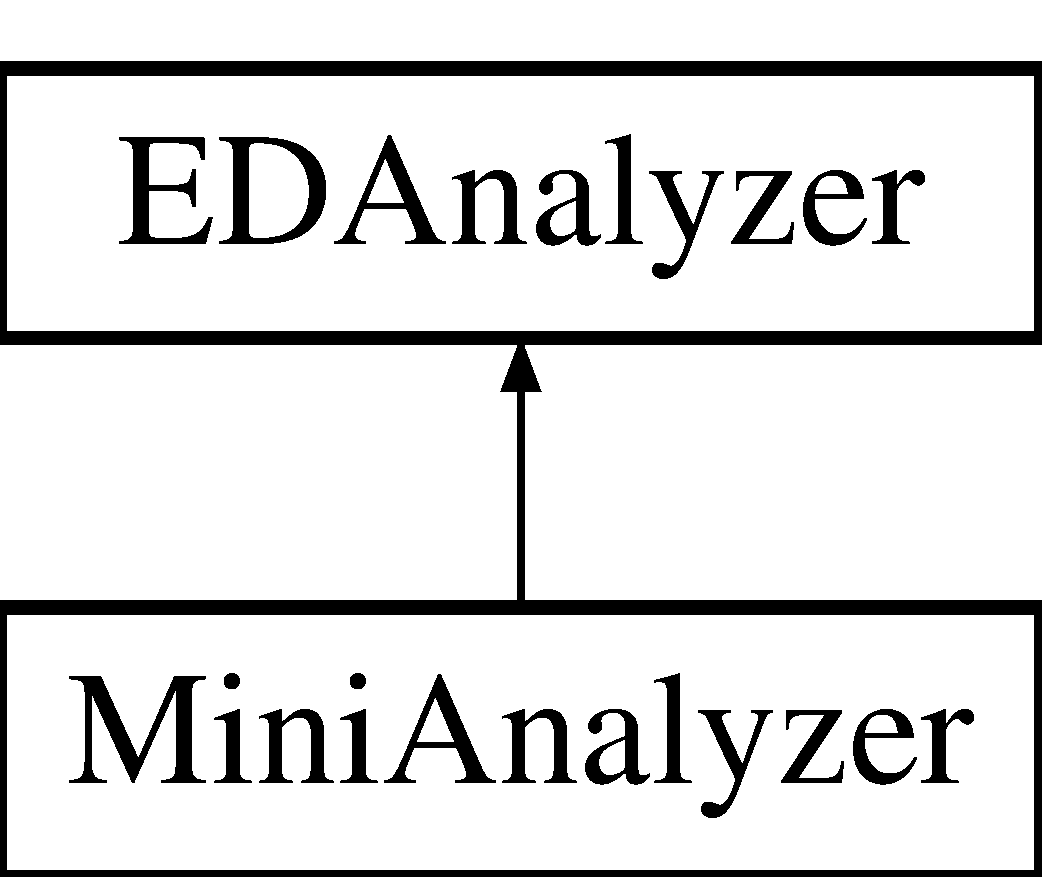
\includegraphics[height=2.000000cm]{classMiniAnalyzer}
\end{center}
\end{figure}
\subsection*{Public Member Functions}
\begin{DoxyCompactItemize}
\item 
\hypertarget{classMiniAnalyzer_af72bdff149b72fdc02f44995b982a778}{{\bfseries Mini\-Analyzer} (const edm\-::\-Parameter\-Set \&)}\label{classMiniAnalyzer_af72bdff149b72fdc02f44995b982a778}

\end{DoxyCompactItemize}
\subsection*{Static Public Member Functions}
\begin{DoxyCompactItemize}
\item 
\hypertarget{classMiniAnalyzer_a5199abda9815be60babdc07c76fa2c90}{static void {\bfseries fill\-Descriptions} (edm\-::\-Configuration\-Descriptions \&descriptions)}\label{classMiniAnalyzer_a5199abda9815be60babdc07c76fa2c90}

\end{DoxyCompactItemize}


\subsection{Detailed Description}
Description\-: \mbox{[}one line class summary\mbox{]}

Implementation\-: \mbox{[}Notes on implementation\mbox{]} 

The documentation for this class was generated from the following file\-:\begin{DoxyCompactItemize}
\item 
plugins/Mini\-Analyzer.\-cc\end{DoxyCompactItemize}

\hypertarget{structran_1_1MuonStruct}{\section{ran\-:\-:Muon\-Struct Struct Reference}
\label{structran_1_1MuonStruct}\index{ran\-::\-Muon\-Struct@{ran\-::\-Muon\-Struct}}
}
Inheritance diagram for ran\-:\-:Muon\-Struct\-:\begin{figure}[H]
\begin{center}
\leavevmode
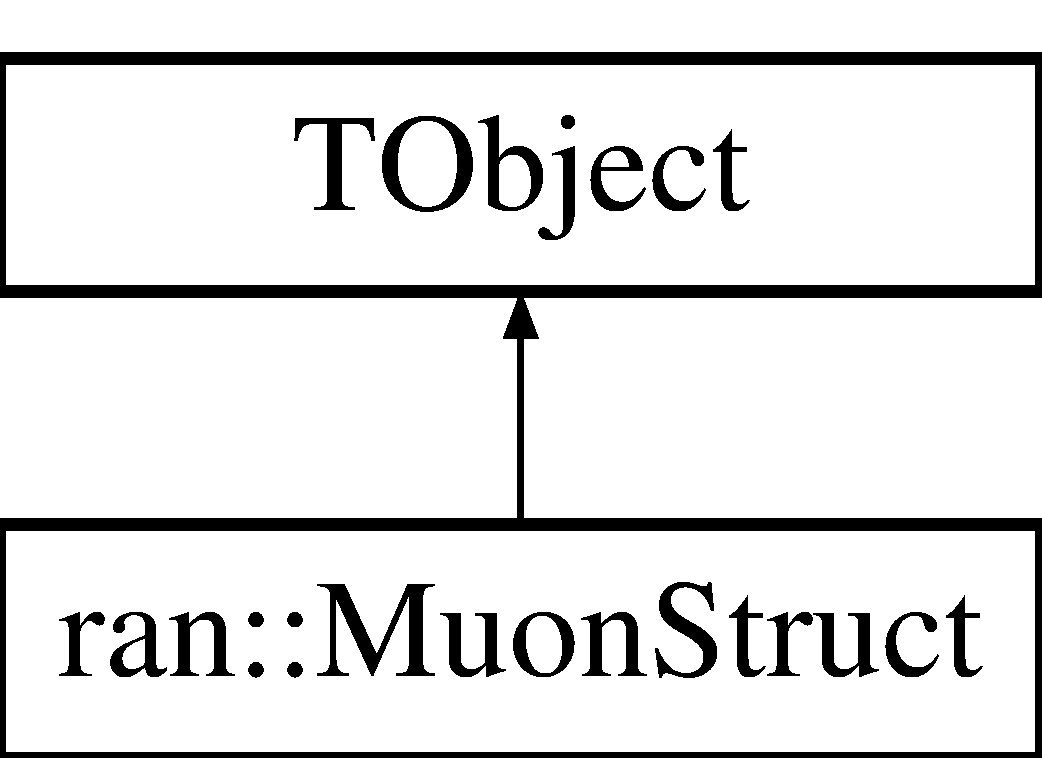
\includegraphics[height=2.000000cm]{structran_1_1MuonStruct}
\end{center}
\end{figure}
\subsection*{Public Member Functions}
\begin{DoxyCompactItemize}
\item 
\hypertarget{structran_1_1MuonStruct_af62411bcdf5d93802b07f06116c8363f}{\hyperlink{structran_1_1MuonStruct_af62411bcdf5d93802b07f06116c8363f}{Muon\-Struct} ()}\label{structran_1_1MuonStruct_af62411bcdf5d93802b07f06116c8363f}

\begin{DoxyCompactList}\small\item\em default constructor \end{DoxyCompactList}\item 
\hypertarget{structran_1_1MuonStruct_a1059cb8528a5e851b4c6566d84634d66}{virtual \hyperlink{structran_1_1MuonStruct_a1059cb8528a5e851b4c6566d84634d66}{$\sim$\-Muon\-Struct} ()}\label{structran_1_1MuonStruct_a1059cb8528a5e851b4c6566d84634d66}

\begin{DoxyCompactList}\small\item\em virtual distructor \end{DoxyCompactList}\end{DoxyCompactItemize}
\subsection*{Public Attributes}
\begin{DoxyCompactItemize}
\item 
\hypertarget{structran_1_1MuonStruct_ae9ed522209187b6eb1993d6fe3ace9e3}{double \hyperlink{structran_1_1MuonStruct_ae9ed522209187b6eb1993d6fe3ace9e3}{pt}}\label{structran_1_1MuonStruct_ae9ed522209187b6eb1993d6fe3ace9e3}

\begin{DoxyCompactList}\small\item\em pt \end{DoxyCompactList}\item 
\hypertarget{structran_1_1MuonStruct_a22bdc36cd92f2b986d76afafb29e0b11}{double \hyperlink{structran_1_1MuonStruct_a22bdc36cd92f2b986d76afafb29e0b11}{eta}}\label{structran_1_1MuonStruct_a22bdc36cd92f2b986d76afafb29e0b11}

\begin{DoxyCompactList}\small\item\em eta \end{DoxyCompactList}\item 
\hypertarget{structran_1_1MuonStruct_a5a90b9ca53b373c65135f6330236772e}{R\-O\-O\-T\-::\-Math\-::\-X\-Y\-Z\-T\-Vector {\bfseries p4}}\label{structran_1_1MuonStruct_a5a90b9ca53b373c65135f6330236772e}

\item 
\hypertarget{structran_1_1MuonStruct_a14950f7d1af0a251cebb257322533892}{int {\bfseries charge}}\label{structran_1_1MuonStruct_a14950f7d1af0a251cebb257322533892}

\item 
\hypertarget{structran_1_1MuonStruct_a42a703eab221d7965612bc54a012ebae}{bool {\bfseries is\-Global\-Muon}}\label{structran_1_1MuonStruct_a42a703eab221d7965612bc54a012ebae}

\item 
\hypertarget{structran_1_1MuonStruct_aedb458d1e954e76000f4defb3f9e3bb1}{bool {\bfseries is\-Tracker\-Muon}}\label{structran_1_1MuonStruct_aedb458d1e954e76000f4defb3f9e3bb1}

\item 
\hypertarget{structran_1_1MuonStruct_adc548247ac7b5c93b9a9a9b14f7caa38}{bool {\bfseries is\-Stand\-Alone\-Muon}}\label{structran_1_1MuonStruct_adc548247ac7b5c93b9a9a9b14f7caa38}

\item 
\hypertarget{structran_1_1MuonStruct_a79355eeafd5645899db84e63bbd2efca}{int {\bfseries num\-Matched\-Muon\-Stns}}\label{structran_1_1MuonStruct_a79355eeafd5645899db84e63bbd2efca}

\item 
\hypertarget{structran_1_1MuonStruct_a81fe2d49740b081f440c454ad604dc5a}{double {\bfseries d\-B}}\label{structran_1_1MuonStruct_a81fe2d49740b081f440c454ad604dc5a}

\item 
\hypertarget{structran_1_1MuonStruct_a11da16560788a7cf6a8892d07ba30e53}{bool \hyperlink{structran_1_1MuonStruct_a11da16560788a7cf6a8892d07ba30e53}{is\-P\-F\-Isolation\-Valid}}\label{structran_1_1MuonStruct_a11da16560788a7cf6a8892d07ba30e53}

\begin{DoxyCompactList}\small\item\em Is particle flow isolation valid. \end{DoxyCompactList}\item 
\hypertarget{structran_1_1MuonStruct_a1334f17756d9fcc9a21ff9fc15d4aa74}{double \hyperlink{structran_1_1MuonStruct_a1334f17756d9fcc9a21ff9fc15d4aa74}{pf\-Iso\-R03\-\_\-sum\-Chg\-Had\-Pt}}\label{structran_1_1MuonStruct_a1334f17756d9fcc9a21ff9fc15d4aa74}

\begin{DoxyCompactList}\small\item\em sum-\/pt of charged Hadro \end{DoxyCompactList}\item 
\hypertarget{structran_1_1MuonStruct_a69bc50b0159358e68682b13e2e14cff3}{double \hyperlink{structran_1_1MuonStruct_a69bc50b0159358e68682b13e2e14cff3}{pf\-Iso\-R03\-\_\-chg\-Part\-Pt}}\label{structran_1_1MuonStruct_a69bc50b0159358e68682b13e2e14cff3}

\begin{DoxyCompactList}\small\item\em sum-\/pt of charged Particles(inludes e/mu) \end{DoxyCompactList}\item 
\hypertarget{structran_1_1MuonStruct_a8cb22c69db0b4f9a88898423537decc1}{double \hyperlink{structran_1_1MuonStruct_a8cb22c69db0b4f9a88898423537decc1}{pf\-Iso\-R03\-\_\-sum\-Neut\-Had\-Pt}}\label{structran_1_1MuonStruct_a8cb22c69db0b4f9a88898423537decc1}

\begin{DoxyCompactList}\small\item\em sum pt of neutral hadrons \end{DoxyCompactList}\item 
\hypertarget{structran_1_1MuonStruct_ae300f58260fb97e77206435b36d3fcf6}{double \hyperlink{structran_1_1MuonStruct_ae300f58260fb97e77206435b36d3fcf6}{pf\-Iso\-R03\-\_\-sum\-Pht\-Et}}\label{structran_1_1MuonStruct_ae300f58260fb97e77206435b36d3fcf6}

\begin{DoxyCompactList}\small\item\em sum pt of P\-F photons \end{DoxyCompactList}\item 
\hypertarget{structran_1_1MuonStruct_accae0c44dc80c5e52a22c671479a66d2}{bool \hyperlink{structran_1_1MuonStruct_accae0c44dc80c5e52a22c671479a66d2}{is\-Isolation\-Valid}}\label{structran_1_1MuonStruct_accae0c44dc80c5e52a22c671479a66d2}

\begin{DoxyCompactList}\small\item\em Is isolation valid. \end{DoxyCompactList}\item 
\hypertarget{structran_1_1MuonStruct_aa864a85b3e3d98867f8c9ed945453a32}{double {\bfseries isol\-R03\-\_\-sum\-Pt}}\label{structran_1_1MuonStruct_aa864a85b3e3d98867f8c9ed945453a32}

\item 
\hypertarget{structran_1_1MuonStruct_a8dc18d3385d2e5bf279c0f4cef7b645d}{double {\bfseries isol\-R03\-\_\-em\-Et}}\label{structran_1_1MuonStruct_a8dc18d3385d2e5bf279c0f4cef7b645d}

\item 
\hypertarget{structran_1_1MuonStruct_a892e00a5b9fdfa2b7c84067390bcbb23}{double {\bfseries isol\-R03\-\_\-had\-Et}}\label{structran_1_1MuonStruct_a892e00a5b9fdfa2b7c84067390bcbb23}

\item 
\hypertarget{structran_1_1MuonStruct_acaf6f39facbff0fdeed39686d6dea8e5}{double \hyperlink{structran_1_1MuonStruct_acaf6f39facbff0fdeed39686d6dea8e5}{dxy}}\label{structran_1_1MuonStruct_acaf6f39facbff0fdeed39686d6dea8e5}

\begin{DoxyCompactList}\small\item\em No quality cuts on the vertex. \end{DoxyCompactList}\item 
\hypertarget{structran_1_1MuonStruct_ab768447117d1f94ee92607345a5580e9}{double \hyperlink{structran_1_1MuonStruct_ab768447117d1f94ee92607345a5580e9}{dz}}\label{structran_1_1MuonStruct_ab768447117d1f94ee92607345a5580e9}

\begin{DoxyCompactList}\small\item\em No quality cuts on the vertex. \end{DoxyCompactList}\item 
\hypertarget{structran_1_1MuonStruct_a22bbc7de6d58433950de87b9162d65b2}{bool {\bfseries glob\-Trk\-\_\-exists}}\label{structran_1_1MuonStruct_a22bbc7de6d58433950de87b9162d65b2}

\item 
\hypertarget{structran_1_1MuonStruct_addd01b3681d8829f6a99c5e09e5c6030}{double {\bfseries glob\-Trk\-\_\-p\-T}}\label{structran_1_1MuonStruct_addd01b3681d8829f6a99c5e09e5c6030}

\item 
\hypertarget{structran_1_1MuonStruct_a5c4c2ebb4bd28225b56c54af187757bc}{double {\bfseries glob\-Trk\-\_\-eta}}\label{structran_1_1MuonStruct_a5c4c2ebb4bd28225b56c54af187757bc}

\item 
\hypertarget{structran_1_1MuonStruct_a33a069f3f6f3b8fc910bd12320e32cda}{double {\bfseries glob\-Trk\-\_\-phi}}\label{structran_1_1MuonStruct_a33a069f3f6f3b8fc910bd12320e32cda}

\item 
\hypertarget{structran_1_1MuonStruct_aeeb13a761abe629d490cbf0dd8fbc1b5}{int {\bfseries glob\-Trk\-\_\-charge}}\label{structran_1_1MuonStruct_aeeb13a761abe629d490cbf0dd8fbc1b5}

\item 
\hypertarget{structran_1_1MuonStruct_aa00a2a3376f277412c6ba9a9521f348c}{int {\bfseries glob\-Trk\-\_\-number\-Of\-Valid\-Muon\-Hits}}\label{structran_1_1MuonStruct_aa00a2a3376f277412c6ba9a9521f348c}

\item 
\hypertarget{structran_1_1MuonStruct_abd4d2d0d94fabcfaf4e6db23cafdacac}{double {\bfseries glob\-Trk\-\_\-normalised\-Chi2}}\label{structran_1_1MuonStruct_abd4d2d0d94fabcfaf4e6db23cafdacac}

\item 
\hypertarget{structran_1_1MuonStruct_a85069de493c184137513f9a9bab4b264}{bool {\bfseries in\-Trk\-\_\-exists}}\label{structran_1_1MuonStruct_a85069de493c184137513f9a9bab4b264}

\item 
\hypertarget{structran_1_1MuonStruct_a6866a343bd067caa4456f132d0cbcb07}{double {\bfseries in\-Trk\-\_\-p\-T}}\label{structran_1_1MuonStruct_a6866a343bd067caa4456f132d0cbcb07}

\item 
\hypertarget{structran_1_1MuonStruct_aef4a9cffe92e3d56b4ed86e07d3dac0d}{double {\bfseries in\-Trk\-\_\-eta}}\label{structran_1_1MuonStruct_aef4a9cffe92e3d56b4ed86e07d3dac0d}

\item 
\hypertarget{structran_1_1MuonStruct_a43658eb3784049b68dc33527e5645204}{double {\bfseries in\-Trk\-\_\-phi}}\label{structran_1_1MuonStruct_a43658eb3784049b68dc33527e5645204}

\item 
\hypertarget{structran_1_1MuonStruct_ab93502c5e1eff3a42cc44b732a1cb5b0}{int {\bfseries in\-Trk\-\_\-charge}}\label{structran_1_1MuonStruct_ab93502c5e1eff3a42cc44b732a1cb5b0}

\item 
\hypertarget{structran_1_1MuonStruct_a710e8c5f85111b976783e4b816e09723}{int {\bfseries in\-Trk\-\_\-num\-Valid\-Pix\-Hits}}\label{structran_1_1MuonStruct_a710e8c5f85111b976783e4b816e09723}

\item 
\hypertarget{structran_1_1MuonStruct_aeb3cd4af54d1dc0d4c4062fa14d4bc13}{int {\bfseries in\-Trk\-\_\-num\-Valid\-Trkr\-Hits}}\label{structran_1_1MuonStruct_aeb3cd4af54d1dc0d4c4062fa14d4bc13}

\item 
\hypertarget{structran_1_1MuonStruct_a24069ce9b716d399e061f25c9f69b190}{double {\bfseries in\-Trk\-\_\-tracker\-Layers\-With\-Measurement}}\label{structran_1_1MuonStruct_a24069ce9b716d399e061f25c9f69b190}

\item 
\hypertarget{structran_1_1MuonStruct_ab8eeecd4c250485829a23370706237af}{double {\bfseries in\-Trk\-\_\-dxy\-Vs\-Origin}}\label{structran_1_1MuonStruct_ab8eeecd4c250485829a23370706237af}

\item 
\hypertarget{structran_1_1MuonStruct_a4d6a52fd6bde6616d5312a19c7fb20da}{int {\bfseries trk\-\_\-trkr\-Layers\-W\-Hits}}\label{structran_1_1MuonStruct_a4d6a52fd6bde6616d5312a19c7fb20da}

\item 
\hypertarget{structran_1_1MuonStruct_a4b8e7968d395bcf3c5611014f7884c1d}{bool {\bfseries out\-Trk\-\_\-exists}}\label{structran_1_1MuonStruct_a4b8e7968d395bcf3c5611014f7884c1d}

\item 
\hypertarget{structran_1_1MuonStruct_a6928c3f5b98746a8381f5ffa96ec2c32}{double {\bfseries out\-Trk\-\_\-p\-T}}\label{structran_1_1MuonStruct_a6928c3f5b98746a8381f5ffa96ec2c32}

\item 
\hypertarget{structran_1_1MuonStruct_a3b7741a7d37f3ea3cd3b60ded50ad852}{double {\bfseries out\-Trk\-\_\-eta}}\label{structran_1_1MuonStruct_a3b7741a7d37f3ea3cd3b60ded50ad852}

\item 
\hypertarget{structran_1_1MuonStruct_ad9ac8db0b546acce3f263f0a7788696c}{double {\bfseries out\-Trk\-\_\-phi}}\label{structran_1_1MuonStruct_ad9ac8db0b546acce3f263f0a7788696c}

\item 
\hypertarget{structran_1_1MuonStruct_a58dc3402fde305d06acd86449811c4c1}{int {\bfseries out\-Trk\-\_\-charge}}\label{structran_1_1MuonStruct_a58dc3402fde305d06acd86449811c4c1}

\item 
\hypertarget{structran_1_1MuonStruct_ad581563fb43f247732faf3a68465c8c0}{bool {\bfseries best\-Trk\-\_\-exists}}\label{structran_1_1MuonStruct_ad581563fb43f247732faf3a68465c8c0}

\item 
\hypertarget{structran_1_1MuonStruct_addafb3644a63febae06934f3c99ca096}{double {\bfseries best\-Trk\-\_\-dxy\-\_\-bspot}}\label{structran_1_1MuonStruct_addafb3644a63febae06934f3c99ca096}

\item 
\hypertarget{structran_1_1MuonStruct_aa87351db95884e37556cf7030a86bccc}{double {\bfseries best\-Trk\-\_\-dxy\-\_\-vtx}}\label{structran_1_1MuonStruct_aa87351db95884e37556cf7030a86bccc}

\item 
\hypertarget{structran_1_1MuonStruct_abb9ab8ee0219e1db5c72d3c7e8dcb835}{double {\bfseries best\-Trk\-\_\-dz\-\_\-vtx}}\label{structran_1_1MuonStruct_abb9ab8ee0219e1db5c72d3c7e8dcb835}

\end{DoxyCompactItemize}


The documentation for this struct was generated from the following files\-:\begin{DoxyCompactItemize}
\item 
interface/Muon\-Struct.\-hh\item 
src/Muon\-Struct.\-cc\end{DoxyCompactItemize}

\hypertarget{classran_1_1NtElectron}{\section{ran\-:\-:Nt\-Electron Class Reference}
\label{classran_1_1NtElectron}\index{ran\-::\-Nt\-Electron@{ran\-::\-Nt\-Electron}}
}
\subsection*{Public Member Functions}
\begin{DoxyCompactItemize}
\item 
\hypertarget{classran_1_1NtElectron_a9894bfecb290959cf63dc7b7b5b937db}{\hyperlink{classran_1_1NtElectron_a9894bfecb290959cf63dc7b7b5b937db}{Nt\-Electron} ()}\label{classran_1_1NtElectron_a9894bfecb290959cf63dc7b7b5b937db}

\begin{DoxyCompactList}\small\item\em Default constructor. \end{DoxyCompactList}\item 
\hypertarget{classran_1_1NtElectron_a10786baddcc09f56a22ac11daa274416}{\hyperlink{classran_1_1NtElectron_a10786baddcc09f56a22ac11daa274416}{Nt\-Electron} (const \hyperlink{classran_1_1ElectronStruct}{ran\-::\-Electron\-Struct} \&an\-Electron)}\label{classran_1_1NtElectron_a10786baddcc09f56a22ac11daa274416}

\begin{DoxyCompactList}\small\item\em Constructor. \end{DoxyCompactList}\item 
\hypertarget{classran_1_1NtElectron_a9707f61ec74a898532aa8ec84c31d075}{double \hyperlink{classran_1_1NtElectron_a9707f61ec74a898532aa8ec84c31d075}{pt} () const }\label{classran_1_1NtElectron_a9707f61ec74a898532aa8ec84c31d075}

\begin{DoxyCompactList}\small\item\em Particle pt. \end{DoxyCompactList}\item 
\hypertarget{classran_1_1NtElectron_aa270b767101d46ee92711dce9d1ba47e}{double \hyperlink{classran_1_1NtElectron_aa270b767101d46ee92711dce9d1ba47e}{eta} () const }\label{classran_1_1NtElectron_aa270b767101d46ee92711dce9d1ba47e}

\begin{DoxyCompactList}\small\item\em Particle eta. \end{DoxyCompactList}\item 
\hypertarget{classran_1_1NtElectron_a0337d765a1985f4a87a26061e0cf898e}{bool \hyperlink{classran_1_1NtElectron_a0337d765a1985f4a87a26061e0cf898e}{gsf\-Track\-\_\-available} () const }\label{classran_1_1NtElectron_a0337d765a1985f4a87a26061e0cf898e}

\begin{DoxyCompactList}\small\item\em Is G\-S\-F track available. \end{DoxyCompactList}\item 
\hypertarget{classran_1_1NtElectron_a8aedba5b827dcc122516cb166c41cd37}{double \hyperlink{classran_1_1NtElectron_a8aedba5b827dcc122516cb166c41cd37}{sc\-Eta} () const }\label{classran_1_1NtElectron_a8aedba5b827dcc122516cb166c41cd37}

\begin{DoxyCompactList}\small\item\em super cluster eta \end{DoxyCompactList}\item 
\hypertarget{classran_1_1NtElectron_afdd479d9ffa3f26240b6c450856b20ba}{double \hyperlink{classran_1_1NtElectron_afdd479d9ffa3f26240b6c450856b20ba}{sc\-Energy} () const }\label{classran_1_1NtElectron_afdd479d9ffa3f26240b6c450856b20ba}

\begin{DoxyCompactList}\small\item\em super cluster energy \end{DoxyCompactList}\item 
\hypertarget{classran_1_1NtElectron_a896afa5c6fb469f466ef547f6a50dd2e}{bool \hyperlink{classran_1_1NtElectron_a896afa5c6fb469f466ef547f6a50dd2e}{ecal\-Driven\-Seed} () const }\label{classran_1_1NtElectron_a896afa5c6fb469f466ef547f6a50dd2e}

\begin{DoxyCompactList}\small\item\em is ecal driven \end{DoxyCompactList}\item 
\hypertarget{classran_1_1NtElectron_a36c82cd5578080677b9b286e80108aca}{double \hyperlink{classran_1_1NtElectron_a36c82cd5578080677b9b286e80108aca}{e2x5\-Max} () const }\label{classran_1_1NtElectron_a36c82cd5578080677b9b286e80108aca}

\begin{DoxyCompactList}\small\item\em e2x5 max \end{DoxyCompactList}\item 
\hypertarget{classran_1_1NtElectron_a869a9ce218bbed37bb47b9ff674efdee}{double \hyperlink{classran_1_1NtElectron_a869a9ce218bbed37bb47b9ff674efdee}{e5x5} () const }\label{classran_1_1NtElectron_a869a9ce218bbed37bb47b9ff674efdee}

\begin{DoxyCompactList}\small\item\em e5x5 \end{DoxyCompactList}\item 
\hypertarget{classran_1_1NtElectron_ad4fa44f1651a86189547992a49cb5a26}{double \hyperlink{classran_1_1NtElectron_ad4fa44f1651a86189547992a49cb5a26}{e1x5} () const }\label{classran_1_1NtElectron_ad4fa44f1651a86189547992a49cb5a26}

\begin{DoxyCompactList}\small\item\em e1x5 \end{DoxyCompactList}\item 
\hypertarget{classran_1_1NtElectron_a7ee65cf4cdf115cbafba25f901dad0ff}{double {\bfseries delta\-Phi\-Super\-Cluster\-Track\-At\-Vtx} () const }\label{classran_1_1NtElectron_a7ee65cf4cdf115cbafba25f901dad0ff}

\item 
\hypertarget{classran_1_1NtElectron_a89fb13136b948d50e34f8430c060241a}{double \hyperlink{classran_1_1NtElectron_a89fb13136b948d50e34f8430c060241a}{hadronic\-Over\-Em} () const }\label{classran_1_1NtElectron_a89fb13136b948d50e34f8430c060241a}

\begin{DoxyCompactList}\small\item\em H/\-E. \end{DoxyCompactList}\item 
\hypertarget{classran_1_1NtElectron_a056954295bfc2e8ed4f42d417e4a2a47}{double {\bfseries sc\-Sigma\-I\-Eta\-I\-Eta} () const }\label{classran_1_1NtElectron_a056954295bfc2e8ed4f42d417e4a2a47}

\item 
\hypertarget{classran_1_1NtElectron_adf42db8afac88f64cc158c321ebe7001}{double {\bfseries dr03\-Ecal\-Rec\-Hit\-Sum\-Et} () const }\label{classran_1_1NtElectron_adf42db8afac88f64cc158c321ebe7001}

\item 
\hypertarget{classran_1_1NtElectron_a9c5a0f9beb630fdd9ba0bd283e51e267}{double {\bfseries dr03\-Hcal\-Depth1\-Tower\-Sum\-Et} () const }\label{classran_1_1NtElectron_a9c5a0f9beb630fdd9ba0bd283e51e267}

\item 
\hypertarget{classran_1_1NtElectron_a17fef20cad5536dd731fbd18118e0b6c}{double {\bfseries dr03\-Tk\-Sum\-Pt} () const }\label{classran_1_1NtElectron_a17fef20cad5536dd731fbd18118e0b6c}

\item 
\hypertarget{classran_1_1NtElectron_a7f2fa48a46960372c6db4ae71cee6c03}{double \hyperlink{classran_1_1NtElectron_a7f2fa48a46960372c6db4ae71cee6c03}{sigma\-Ieta\-Ieta} () const }\label{classran_1_1NtElectron_a7f2fa48a46960372c6db4ae71cee6c03}

\begin{DoxyCompactList}\small\item\em sigma\-Ieta\-Ieta \end{DoxyCompactList}\item 
\hypertarget{classran_1_1NtElectron_a7a4a2732c47bc01638a0e509a2d5e7c9}{double \hyperlink{classran_1_1NtElectron_a7a4a2732c47bc01638a0e509a2d5e7c9}{full5x5\-\_\-sigma\-Ieta\-Ieta} () const }\label{classran_1_1NtElectron_a7a4a2732c47bc01638a0e509a2d5e7c9}

\begin{DoxyCompactList}\small\item\em full5x5\-\_\-sigma\-Ieta\-Ieta \end{DoxyCompactList}\item 
\hypertarget{classran_1_1NtElectron_aed16a4122778a43e1d6e9607130e6e7e}{bool \hyperlink{classran_1_1NtElectron_aed16a4122778a43e1d6e9607130e6e7e}{pass\-Conversion\-Veto} () const }\label{classran_1_1NtElectron_aed16a4122778a43e1d6e9607130e6e7e}

\begin{DoxyCompactList}\small\item\em pass\-Conversion\-Veto \end{DoxyCompactList}\end{DoxyCompactItemize}


The documentation for this class was generated from the following file\-:\begin{DoxyCompactItemize}
\item 
interface/Nt\-Electron.\-hh\end{DoxyCompactItemize}

\hypertarget{classran_1_1NtJet}{\section{ran\-:\-:Nt\-Jet Class Reference}
\label{classran_1_1NtJet}\index{ran\-::\-Nt\-Jet@{ran\-::\-Nt\-Jet}}
}
\subsection*{Public Member Functions}
\begin{DoxyCompactItemize}
\item 
\hypertarget{classran_1_1NtJet_a40c6162763747a9353ba0cc36d4f4713}{\hyperlink{classran_1_1NtJet_a40c6162763747a9353ba0cc36d4f4713}{Nt\-Jet} ()}\label{classran_1_1NtJet_a40c6162763747a9353ba0cc36d4f4713}

\begin{DoxyCompactList}\small\item\em Default constructor. \end{DoxyCompactList}\item 
\hypertarget{classran_1_1NtJet_af447af0df9b93fbaf86b306034cc9ea0}{\hyperlink{classran_1_1NtJet_af447af0df9b93fbaf86b306034cc9ea0}{Nt\-Jet} (const \hyperlink{structran_1_1JetStruct}{ran\-::\-Jet\-Struct} \&a\-Jet)}\label{classran_1_1NtJet_af447af0df9b93fbaf86b306034cc9ea0}

\begin{DoxyCompactList}\small\item\em Constructor. \end{DoxyCompactList}\item 
\hypertarget{classran_1_1NtJet_a21823898e1e0afd81c377a065025c3b3}{double \hyperlink{classran_1_1NtJet_a21823898e1e0afd81c377a065025c3b3}{pt} () const }\label{classran_1_1NtJet_a21823898e1e0afd81c377a065025c3b3}

\begin{DoxyCompactList}\small\item\em Particle pt. \end{DoxyCompactList}\item 
\hypertarget{classran_1_1NtJet_ac934581307c87c5195272ad4e849d29f}{double \hyperlink{classran_1_1NtJet_ac934581307c87c5195272ad4e849d29f}{et} () const }\label{classran_1_1NtJet_ac934581307c87c5195272ad4e849d29f}

\begin{DoxyCompactList}\small\item\em Particle et. \end{DoxyCompactList}\item 
\hypertarget{classran_1_1NtJet_ac4fef92d0097c092069b5a82daa2c3ae}{double \hyperlink{classran_1_1NtJet_ac4fef92d0097c092069b5a82daa2c3ae}{eta} () const }\label{classran_1_1NtJet_ac4fef92d0097c092069b5a82daa2c3ae}

\begin{DoxyCompactList}\small\item\em Particle eta. \end{DoxyCompactList}\item 
\hypertarget{classran_1_1NtJet_a79d3419ba9701c4170f1dc4104b24867}{double \hyperlink{classran_1_1NtJet_a79d3419ba9701c4170f1dc4104b24867}{mass} () const }\label{classran_1_1NtJet_a79d3419ba9701c4170f1dc4104b24867}

\begin{DoxyCompactList}\small\item\em Particle mass. \end{DoxyCompactList}\item 
\hypertarget{classran_1_1NtJet_a48a59bb320e43ed9130bad31bac4bf37}{double \hyperlink{classran_1_1NtJet_a48a59bb320e43ed9130bad31bac4bf37}{jet\-Probability\-B\-Jet\-Tags} () const }\label{classran_1_1NtJet_a48a59bb320e43ed9130bad31bac4bf37}

\begin{DoxyCompactList}\small\item\em jet\-Probability\-B\-Jet\-Tags b tag discriminator \end{DoxyCompactList}\item 
\hypertarget{classran_1_1NtJet_af04bcd597fa9d1c124821e3db7ad3c4f}{double \hyperlink{classran_1_1NtJet_af04bcd597fa9d1c124821e3db7ad3c4f}{jet\-B\-Probability\-B\-Jet\-Tags} () const }\label{classran_1_1NtJet_af04bcd597fa9d1c124821e3db7ad3c4f}

\begin{DoxyCompactList}\small\item\em jet\-B\-Probability\-B\-Jet\-Tags b tag discriminator \end{DoxyCompactList}\item 
\hypertarget{classran_1_1NtJet_ade84ff4ae60e81b5029d7e18e49a9ef0}{double \hyperlink{classran_1_1NtJet_ade84ff4ae60e81b5029d7e18e49a9ef0}{track\-Counting\-High\-Eff\-B\-Jet\-Tags} () const }\label{classran_1_1NtJet_ade84ff4ae60e81b5029d7e18e49a9ef0}

\begin{DoxyCompactList}\small\item\em track\-Counting\-High\-Eff\-B\-Jet\-Tags b tag discriminator \end{DoxyCompactList}\item 
\hypertarget{classran_1_1NtJet_a0c608fa459cc69f38cb9bb869ab883c5}{double \hyperlink{classran_1_1NtJet_a0c608fa459cc69f38cb9bb869ab883c5}{track\-Counting\-High\-Pur\-B\-Jet\-Tags} () const }\label{classran_1_1NtJet_a0c608fa459cc69f38cb9bb869ab883c5}

\begin{DoxyCompactList}\small\item\em track\-Counting\-High\-Pur\-B\-Jet\-Tags b tag discriminator \end{DoxyCompactList}\item 
\hypertarget{classran_1_1NtJet_a802d3c0f4d9bed5c98c7cceff8632599}{double \hyperlink{classran_1_1NtJet_a802d3c0f4d9bed5c98c7cceff8632599}{simple\-Secondary\-Vertex\-High\-Eff\-B\-Jet\-Tags} () const }\label{classran_1_1NtJet_a802d3c0f4d9bed5c98c7cceff8632599}

\begin{DoxyCompactList}\small\item\em simple\-Secondary\-Vertex\-High\-Eff\-B\-Jet\-Tags b tag discriminator \end{DoxyCompactList}\item 
\hypertarget{classran_1_1NtJet_a64b9c27a1a33fd9345b8711c62ef04dd}{double \hyperlink{classran_1_1NtJet_a64b9c27a1a33fd9345b8711c62ef04dd}{simple\-Secondary\-Vertex\-High\-Pur\-B\-Jet\-Tags} () const }\label{classran_1_1NtJet_a64b9c27a1a33fd9345b8711c62ef04dd}

\begin{DoxyCompactList}\small\item\em simple\-Secondary\-Vertex\-High\-Pur\-B\-Jet\-Tags b tag discriminator \end{DoxyCompactList}\item 
\hypertarget{classran_1_1NtJet_ad308766f159b857b5347cc8e0274ab56}{double \hyperlink{classran_1_1NtJet_ad308766f159b857b5347cc8e0274ab56}{combined\-Inclusive\-Secondary\-Vertex\-B\-Jet\-Tags} () const }\label{classran_1_1NtJet_ad308766f159b857b5347cc8e0274ab56}

\begin{DoxyCompactList}\small\item\em combined\-Inclusive\-Secondary\-Vertex\-B\-Jet\-Tags b tag discriminator \end{DoxyCompactList}\item 
\hypertarget{classran_1_1NtJet_a896d1123cdaa0ef4ba22246c97ba0972}{double \hyperlink{classran_1_1NtJet_a896d1123cdaa0ef4ba22246c97ba0972}{jec\-Factor\-\_\-un\-Corrected} () const }\label{classran_1_1NtJet_a896d1123cdaa0ef4ba22246c97ba0972}

\begin{DoxyCompactList}\small\item\em factor applied to jet pt to get uncorrect jet pt \end{DoxyCompactList}\item 
\hypertarget{classran_1_1NtJet_a23d9226dd24b48ba16afc96c59a7bbdd}{double \hyperlink{classran_1_1NtJet_a23d9226dd24b48ba16afc96c59a7bbdd}{user\-Float\-\_\-pileup\-Jet\-Id\-\_\-full\-Discriminant} () const }\label{classran_1_1NtJet_a23d9226dd24b48ba16afc96c59a7bbdd}

\begin{DoxyCompactList}\small\item\em user\-Float pileup jet I\-D \end{DoxyCompactList}\item 
\hypertarget{classran_1_1NtJet_aabf92851c5d4855b03028f9f6c5cbdd9}{int \hyperlink{classran_1_1NtJet_aabf92851c5d4855b03028f9f6c5cbdd9}{parton\-Flavour} () const }\label{classran_1_1NtJet_aabf92851c5d4855b03028f9f6c5cbdd9}

\begin{DoxyCompactList}\small\item\em M\-C parton flavour (sensible values for M\-C only!) \end{DoxyCompactList}\end{DoxyCompactItemize}


The documentation for this class was generated from the following file\-:\begin{DoxyCompactItemize}
\item 
interface/Nt\-Jet.\-hh\end{DoxyCompactItemize}

\hypertarget{classran_1_1NtMuon}{\section{ran\-:\-:Nt\-Muon Class Reference}
\label{classran_1_1NtMuon}\index{ran\-::\-Nt\-Muon@{ran\-::\-Nt\-Muon}}
}
\subsection*{Public Member Functions}
\begin{DoxyCompactItemize}
\item 
\hypertarget{classran_1_1NtMuon_a0f5e42b500d8a5f99a6cec3737208a23}{\hyperlink{classran_1_1NtMuon_a0f5e42b500d8a5f99a6cec3737208a23}{Nt\-Muon} ()}\label{classran_1_1NtMuon_a0f5e42b500d8a5f99a6cec3737208a23}

\begin{DoxyCompactList}\small\item\em Default constructor. \end{DoxyCompactList}\item 
\hypertarget{classran_1_1NtMuon_aa29eeb9e98f142ac9b3d135b853f40ea}{\hyperlink{classran_1_1NtMuon_aa29eeb9e98f142ac9b3d135b853f40ea}{Nt\-Muon} (const \hyperlink{structran_1_1MuonStruct}{ran\-::\-Muon\-Struct} \&a\-Muon)}\label{classran_1_1NtMuon_aa29eeb9e98f142ac9b3d135b853f40ea}

\begin{DoxyCompactList}\small\item\em Constructor. \end{DoxyCompactList}\item 
\hypertarget{classran_1_1NtMuon_a728cca4c8275292266356b31ad6068df}{double \hyperlink{classran_1_1NtMuon_a728cca4c8275292266356b31ad6068df}{pt} () const }\label{classran_1_1NtMuon_a728cca4c8275292266356b31ad6068df}

\begin{DoxyCompactList}\small\item\em Particle pt. \end{DoxyCompactList}\item 
\hypertarget{classran_1_1NtMuon_a45af4461d15632c21d3c97ec3183c6dc}{double \hyperlink{classran_1_1NtMuon_a45af4461d15632c21d3c97ec3183c6dc}{eta} () const }\label{classran_1_1NtMuon_a45af4461d15632c21d3c97ec3183c6dc}

\begin{DoxyCompactList}\small\item\em Particle eta. \end{DoxyCompactList}\item 
\hypertarget{classran_1_1NtMuon_abec703d904fd3969dec4d8514cf5cf77}{R\-O\-O\-T\-::\-Math\-::\-X\-Y\-Z\-T\-Vector {\bfseries p4} () const }\label{classran_1_1NtMuon_abec703d904fd3969dec4d8514cf5cf77}

\item 
\hypertarget{classran_1_1NtMuon_a28680d4e5804f296327f901453f78ac6}{int {\bfseries charge} () const }\label{classran_1_1NtMuon_a28680d4e5804f296327f901453f78ac6}

\item 
\hypertarget{classran_1_1NtMuon_ad1b2ca58f3d121f75da6db54a811d5b9}{bool {\bfseries is\-Global\-Muon} () const }\label{classran_1_1NtMuon_ad1b2ca58f3d121f75da6db54a811d5b9}

\item 
\hypertarget{classran_1_1NtMuon_a3ab3cadf47e39ddb4029d9718a3fce7b}{bool {\bfseries is\-Tracker\-Muon} () const }\label{classran_1_1NtMuon_a3ab3cadf47e39ddb4029d9718a3fce7b}

\item 
\hypertarget{classran_1_1NtMuon_a5ad43093658aa1224e0667524e9abbe5}{bool {\bfseries is\-Stand\-Alone\-Muon} () const }\label{classran_1_1NtMuon_a5ad43093658aa1224e0667524e9abbe5}

\item 
\hypertarget{classran_1_1NtMuon_ab375893835b69ae669bf942c64cb5eee}{int {\bfseries num\-Matched\-Muon\-Stns} () const }\label{classran_1_1NtMuon_ab375893835b69ae669bf942c64cb5eee}

\item 
\hypertarget{classran_1_1NtMuon_abf2c67802d6532363945579ccd02b98a}{bool \hyperlink{classran_1_1NtMuon_abf2c67802d6532363945579ccd02b98a}{is\-P\-F\-Isolation\-Valid} () const }\label{classran_1_1NtMuon_abf2c67802d6532363945579ccd02b98a}

\begin{DoxyCompactList}\small\item\em Is particle flow isolation valid. \end{DoxyCompactList}\item 
\hypertarget{classran_1_1NtMuon_a1b052f20279443be34e9a537c2b02abf}{double \hyperlink{classran_1_1NtMuon_a1b052f20279443be34e9a537c2b02abf}{pf\-Iso\-R03\-\_\-sum\-Chg\-Had\-Pt} () const }\label{classran_1_1NtMuon_a1b052f20279443be34e9a537c2b02abf}

\begin{DoxyCompactList}\small\item\em sum-\/pt of charged Hadro \end{DoxyCompactList}\item 
\hypertarget{classran_1_1NtMuon_adce7ac88c61f974c1a5f321327fbcf18}{double \hyperlink{classran_1_1NtMuon_adce7ac88c61f974c1a5f321327fbcf18}{pf\-Iso\-R03\-\_\-chg\-Part\-Pt} () const }\label{classran_1_1NtMuon_adce7ac88c61f974c1a5f321327fbcf18}

\begin{DoxyCompactList}\small\item\em sum-\/pt of charged Particles(inludes e/mu) \end{DoxyCompactList}\item 
\hypertarget{classran_1_1NtMuon_ad7f4522d5f19de0f6009204fc86b5035}{double \hyperlink{classran_1_1NtMuon_ad7f4522d5f19de0f6009204fc86b5035}{pf\-Iso\-R03\-\_\-sum\-Neut\-Had\-Pt} () const }\label{classran_1_1NtMuon_ad7f4522d5f19de0f6009204fc86b5035}

\begin{DoxyCompactList}\small\item\em sum pt of neutral hadrons \end{DoxyCompactList}\item 
\hypertarget{classran_1_1NtMuon_ac68315b6c5e92ab672b6d3592a1a5bc0}{double \hyperlink{classran_1_1NtMuon_ac68315b6c5e92ab672b6d3592a1a5bc0}{pf\-Iso\-R03\-\_\-sum\-Pht\-Et} () const }\label{classran_1_1NtMuon_ac68315b6c5e92ab672b6d3592a1a5bc0}

\begin{DoxyCompactList}\small\item\em sum pt of P\-F photons \end{DoxyCompactList}\item 
\hypertarget{classran_1_1NtMuon_a604415764367bc7635a9be200109deba}{bool \hyperlink{classran_1_1NtMuon_a604415764367bc7635a9be200109deba}{is\-Isolation\-Valid} () const }\label{classran_1_1NtMuon_a604415764367bc7635a9be200109deba}

\begin{DoxyCompactList}\small\item\em Is isolation valid. \end{DoxyCompactList}\item 
\hypertarget{classran_1_1NtMuon_afc8b2c7596fc44d0faa73fb0ecaad0fc}{double {\bfseries isol\-R03\-\_\-sum\-Pt} () const }\label{classran_1_1NtMuon_afc8b2c7596fc44d0faa73fb0ecaad0fc}

\item 
\hypertarget{classran_1_1NtMuon_a280e066cdfea832c19118c9688613c13}{double {\bfseries isol\-R03\-\_\-em\-Et} () const }\label{classran_1_1NtMuon_a280e066cdfea832c19118c9688613c13}

\item 
\hypertarget{classran_1_1NtMuon_a7f6fcc9fa3bfc571ed148cd4f0ada25e}{double {\bfseries isol\-R03\-\_\-had\-Et} () const }\label{classran_1_1NtMuon_a7f6fcc9fa3bfc571ed148cd4f0ada25e}

\item 
\hypertarget{classran_1_1NtMuon_a16cac652ba76f04403bf90933be87626}{double \hyperlink{classran_1_1NtMuon_a16cac652ba76f04403bf90933be87626}{dxy} () const }\label{classran_1_1NtMuon_a16cac652ba76f04403bf90933be87626}

\begin{DoxyCompactList}\small\item\em No quality cuts on the primary vertex. \end{DoxyCompactList}\item 
\hypertarget{classran_1_1NtMuon_a4f501dcc23f456081607fa21f3041301}{double \hyperlink{classran_1_1NtMuon_a4f501dcc23f456081607fa21f3041301}{dz} () const }\label{classran_1_1NtMuon_a4f501dcc23f456081607fa21f3041301}

\begin{DoxyCompactList}\small\item\em No quality cuts on the primary vertex. \end{DoxyCompactList}\item 
\hypertarget{classran_1_1NtMuon_a54d3c69b891096a52ad73dce6346f22b}{bool {\bfseries glob\-Trk\-\_\-exists} () const }\label{classran_1_1NtMuon_a54d3c69b891096a52ad73dce6346f22b}

\item 
\hypertarget{classran_1_1NtMuon_a294f6cbd1342feca13b2afe9875187cf}{double {\bfseries glob\-Trk\-\_\-p\-T} () const }\label{classran_1_1NtMuon_a294f6cbd1342feca13b2afe9875187cf}

\item 
\hypertarget{classran_1_1NtMuon_a175afe8b4884fce3342f0d9ed0d21c4e}{double {\bfseries glob\-Trk\-\_\-eta} () const }\label{classran_1_1NtMuon_a175afe8b4884fce3342f0d9ed0d21c4e}

\item 
\hypertarget{classran_1_1NtMuon_abe59771bb167d0bc3a71281a9d47b6c9}{double {\bfseries glob\-Trk\-\_\-phi} () const }\label{classran_1_1NtMuon_abe59771bb167d0bc3a71281a9d47b6c9}

\item 
\hypertarget{classran_1_1NtMuon_ad8220bcf234147c246db60029c027f1e}{int {\bfseries glob\-Trk\-\_\-charge} () const }\label{classran_1_1NtMuon_ad8220bcf234147c246db60029c027f1e}

\item 
\hypertarget{classran_1_1NtMuon_a18290e4a76a4af9f18a99159e3a11f1d}{int {\bfseries glob\-Trk\-\_\-number\-Of\-Valid\-Muon\-Hits} () const }\label{classran_1_1NtMuon_a18290e4a76a4af9f18a99159e3a11f1d}

\item 
\hypertarget{classran_1_1NtMuon_aaef9c3db9b4db48583dbd0308443b328}{double {\bfseries glob\-Trk\-\_\-normalised\-Chi2} () const }\label{classran_1_1NtMuon_aaef9c3db9b4db48583dbd0308443b328}

\item 
\hypertarget{classran_1_1NtMuon_a312847758a568ca1df115919c4729b8f}{bool {\bfseries in\-Trk\-\_\-exists} () const }\label{classran_1_1NtMuon_a312847758a568ca1df115919c4729b8f}

\item 
\hypertarget{classran_1_1NtMuon_aa992d32d65af13e198acd78754269e0b}{double {\bfseries in\-Trk\-\_\-p\-T} () const }\label{classran_1_1NtMuon_aa992d32d65af13e198acd78754269e0b}

\item 
\hypertarget{classran_1_1NtMuon_a5980458f2138d1e87b97f2ac4ee21cb1}{double {\bfseries in\-Trk\-\_\-eta} () const }\label{classran_1_1NtMuon_a5980458f2138d1e87b97f2ac4ee21cb1}

\item 
\hypertarget{classran_1_1NtMuon_ab6450f1784cadd6f5bbf702791b2da38}{double {\bfseries in\-Trk\-\_\-phi} () const }\label{classran_1_1NtMuon_ab6450f1784cadd6f5bbf702791b2da38}

\item 
\hypertarget{classran_1_1NtMuon_a48c00577d540b79894895681db169fda}{int {\bfseries in\-Trk\-\_\-charge} () const }\label{classran_1_1NtMuon_a48c00577d540b79894895681db169fda}

\item 
\hypertarget{classran_1_1NtMuon_a933123e54df9e15bac1de6bdfa3b5784}{int {\bfseries in\-Trk\-\_\-num\-Valid\-Pix\-Hits} () const }\label{classran_1_1NtMuon_a933123e54df9e15bac1de6bdfa3b5784}

\item 
\hypertarget{classran_1_1NtMuon_ac703f7c338834e6c9cb6b452e90dec2b}{int {\bfseries in\-Trk\-\_\-num\-Valid\-Trkr\-Hits} () const }\label{classran_1_1NtMuon_ac703f7c338834e6c9cb6b452e90dec2b}

\item 
\hypertarget{classran_1_1NtMuon_a2607d2f9dc04a07d0e39c7cb67615d1d}{double {\bfseries in\-Trk\-\_\-dxy\-Vs\-Origin} () const }\label{classran_1_1NtMuon_a2607d2f9dc04a07d0e39c7cb67615d1d}

\item 
\hypertarget{classran_1_1NtMuon_a305c0e0cddd4f4e62564ff25864ba288}{int {\bfseries trk\-\_\-trkr\-Layers\-W\-Hits} () const }\label{classran_1_1NtMuon_a305c0e0cddd4f4e62564ff25864ba288}

\item 
\hypertarget{classran_1_1NtMuon_af82d2cdae57591f1c47e12366617a5e3}{bool {\bfseries out\-Trk\-\_\-exists} () const }\label{classran_1_1NtMuon_af82d2cdae57591f1c47e12366617a5e3}

\item 
\hypertarget{classran_1_1NtMuon_a6f42b91c697b086b7ebcc682088df217}{double {\bfseries out\-Trk\-\_\-p\-T} () const }\label{classran_1_1NtMuon_a6f42b91c697b086b7ebcc682088df217}

\item 
\hypertarget{classran_1_1NtMuon_a1067b07c94a3ca9465c11cb9520d3083}{double {\bfseries out\-Trk\-\_\-eta} () const }\label{classran_1_1NtMuon_a1067b07c94a3ca9465c11cb9520d3083}

\item 
\hypertarget{classran_1_1NtMuon_abccf52d1154bbce2c3d6c2b8be7cef14}{double {\bfseries out\-Trk\-\_\-phi} () const }\label{classran_1_1NtMuon_abccf52d1154bbce2c3d6c2b8be7cef14}

\item 
\hypertarget{classran_1_1NtMuon_a06cc92e801672aa0d1c2367b3d9ca1b4}{int {\bfseries out\-Trk\-\_\-charge} () const }\label{classran_1_1NtMuon_a06cc92e801672aa0d1c2367b3d9ca1b4}

\item 
\hypertarget{classran_1_1NtMuon_a5d4bf7c61c5ca90892cdd36b30d89af3}{bool {\bfseries best\-Trk\-\_\-exists} () const }\label{classran_1_1NtMuon_a5d4bf7c61c5ca90892cdd36b30d89af3}

\item 
\hypertarget{classran_1_1NtMuon_a89ca8236ad6aca950dad5dc8f4b2de55}{double \hyperlink{classran_1_1NtMuon_a89ca8236ad6aca950dad5dc8f4b2de55}{best\-Trk\-\_\-dxy\-\_\-bspot} () const }\label{classran_1_1NtMuon_a89ca8236ad6aca950dad5dc8f4b2de55}

\begin{DoxyCompactList}\small\item\em Beamspot vertex used. \end{DoxyCompactList}\item 
\hypertarget{classran_1_1NtMuon_a6eb5575058e32e7a2ec1985dc78c89bc}{double \hyperlink{classran_1_1NtMuon_a6eb5575058e32e7a2ec1985dc78c89bc}{best\-Trk\-\_\-dxy\-\_\-vtx} () const }\label{classran_1_1NtMuon_a6eb5575058e32e7a2ec1985dc78c89bc}

\begin{DoxyCompactList}\small\item\em Quality cuts applied to the primary vertex. \end{DoxyCompactList}\item 
\hypertarget{classran_1_1NtMuon_a71ef775fdb73e20a1536e692d0452a20}{double \hyperlink{classran_1_1NtMuon_a71ef775fdb73e20a1536e692d0452a20}{best\-Trk\-\_\-dz\-\_\-vtx} () const }\label{classran_1_1NtMuon_a71ef775fdb73e20a1536e692d0452a20}

\begin{DoxyCompactList}\small\item\em Quality cuts applied to the primary vertex. \end{DoxyCompactList}\end{DoxyCompactItemize}


The documentation for this class was generated from the following file\-:\begin{DoxyCompactItemize}
\item 
interface/Nt\-Muon.\-hh\end{DoxyCompactItemize}

\hypertarget{classNtpReader}{\section{Ntp\-Reader Class Reference}
\label{classNtpReader}\index{Ntp\-Reader@{Ntp\-Reader}}
}
\subsection*{Public Member Functions}
\begin{DoxyCompactItemize}
\item 
\hypertarget{classNtpReader_af11ecbda21ac8dd55e71103f22ace772}{\hyperlink{classNtpReader_af11ecbda21ac8dd55e71103f22ace772}{Ntp\-Reader} (T\-Tree $\ast$in\-Tree)}\label{classNtpReader_af11ecbda21ac8dd55e71103f22ace772}

\begin{DoxyCompactList}\small\item\em Constructor. \end{DoxyCompactList}\item 
\hyperlink{classNtpReader_a31e2f7a7d23d553bc219e11f2e0c8c43}{Ntp\-Reader} (T\-Tree $\ast$in\-Tree, const T\-String \&branch\-Name)
\item 
\hypertarget{classNtpReader_a562709cebd6681f242e3d61d45a4b10c}{\hyperlink{classNtpReader_a562709cebd6681f242e3d61d45a4b10c}{Ntp\-Reader} (string list\-Of\-Files, string tree\-Name)}\label{classNtpReader_a562709cebd6681f242e3d61d45a4b10c}

\begin{DoxyCompactList}\small\item\em Constructor. \end{DoxyCompactList}\item 
\hypertarget{classNtpReader_aa5ea42a326bcfaa6024810d33249c300}{unsigned int {\bfseries run\-Num} () const }\label{classNtpReader_aa5ea42a326bcfaa6024810d33249c300}

\item 
\hypertarget{classNtpReader_a33826fc73883946d273d5fe0f40be06f}{unsigned int {\bfseries evt\-Num} () const }\label{classNtpReader_a33826fc73883946d273d5fe0f40be06f}

\item 
\hypertarget{classNtpReader_aed39639a2892ce1d7874e74e86f30525}{unsigned int {\bfseries lumi\-Sec} () const }\label{classNtpReader_aed39639a2892ce1d7874e74e86f30525}

\item 
\hypertarget{classNtpReader_acde9dee5818258f9ef2fe62cf5248582}{void \hyperlink{classNtpReader_acde9dee5818258f9ef2fe62cf5248582}{set\-Event\-Info\-Branch} (const T\-String \&branch\-Name)}\label{classNtpReader_acde9dee5818258f9ef2fe62cf5248582}

\begin{DoxyCompactList}\small\item\em Sets the event info branch. \end{DoxyCompactList}\item 
\hypertarget{classNtpReader_a625467bc99cd81f63d4ef73c34bcf26c}{void \hyperlink{classNtpReader_a625467bc99cd81f63d4ef73c34bcf26c}{set\-Entry\-Info} ()}\label{classNtpReader_a625467bc99cd81f63d4ef73c34bcf26c}

\begin{DoxyCompactList}\small\item\em sets the event information \end{DoxyCompactList}\item 
\hypertarget{classNtpReader_a34265ba45134f25e07088d0731890882}{{\footnotesize template$<$typename T , typename U $>$ }\\std\-::vector$<$ T $>$ {\bfseries get\-Particle\-Collection} (const T\-String \&branch\-Name)}\label{classNtpReader_a34265ba45134f25e07088d0731890882}

\item 
\hypertarget{classNtpReader_a8dd674f3e6f47cc330f80cb3012d73c0}{std\-::vector$<$ \hyperlink{classran_1_1NtElectron}{ran\-::\-Nt\-Electron} $>$ {\bfseries test\-Branch2} (const T\-String \&branch\-Name)}\label{classNtpReader_a8dd674f3e6f47cc330f80cb3012d73c0}

\item 
\hypertarget{classNtpReader_a22d356eb785288fd3f6b7505b1c0f4f1}{bool \hyperlink{classNtpReader_a22d356eb785288fd3f6b7505b1c0f4f1}{is\-Last\-Entry} ()}\label{classNtpReader_a22d356eb785288fd3f6b7505b1c0f4f1}

\begin{DoxyCompactList}\small\item\em Checks if last event in the ntuple. \end{DoxyCompactList}\item 
\hypertarget{classNtpReader_ac5efd42974d0c40ae189c8fafe3c0cdc}{unsigned int {\bfseries get\-Last\-Entry} ()}\label{classNtpReader_ac5efd42974d0c40ae189c8fafe3c0cdc}

\item 
\hypertarget{classNtpReader_aaee876d696eb198343478b2c191f1675}{unsigned int \hyperlink{classNtpReader_aaee876d696eb198343478b2c191f1675}{get\-Entry\-Number} () const }\label{classNtpReader_aaee876d696eb198343478b2c191f1675}

\begin{DoxyCompactList}\small\item\em Returns the current event number. \end{DoxyCompactList}\item 
\hypertarget{classNtpReader_a04ccaa20b936feab664f0c207c092de5}{void \hyperlink{classNtpReader_a04ccaa20b936feab664f0c207c092de5}{next\-Entry} ()}\label{classNtpReader_a04ccaa20b936feab664f0c207c092de5}

\begin{DoxyCompactList}\small\item\em Increment to next event and set eventinfo. \end{DoxyCompactList}\item 
\hypertarget{classNtpReader_a943e5eefd0b499331c932541d90d9fd3}{void \hyperlink{classNtpReader_a943e5eefd0b499331c932541d90d9fd3}{rese\-Entry} ()}\label{classNtpReader_a943e5eefd0b499331c932541d90d9fd3}

\begin{DoxyCompactList}\small\item\em Reset to first event and set eventinfo. \end{DoxyCompactList}\item 
\hypertarget{classNtpReader_ab7bee0e570b8fdd32dff91ec1acf3851}{void \hyperlink{classNtpReader_ab7bee0e570b8fdd32dff91ec1acf3851}{set\-Entry\-Number} (unsigned int num\-Value)}\label{classNtpReader_ab7bee0e570b8fdd32dff91ec1acf3851}

\begin{DoxyCompactList}\small\item\em Set the event number and set eventinfo. \end{DoxyCompactList}\end{DoxyCompactItemize}


\subsection{Constructor \& Destructor Documentation}
\hypertarget{classNtpReader_a31e2f7a7d23d553bc219e11f2e0c8c43}{\index{Ntp\-Reader@{Ntp\-Reader}!Ntp\-Reader@{Ntp\-Reader}}
\index{Ntp\-Reader@{Ntp\-Reader}!NtpReader@{Ntp\-Reader}}
\subsubsection[{Ntp\-Reader}]{\setlength{\rightskip}{0pt plus 5cm}Ntp\-Reader\-::\-Ntp\-Reader (
\begin{DoxyParamCaption}
\item[{T\-Tree $\ast$}]{in\-Tree, }
\item[{const T\-String \&}]{branch\-Name}
\end{DoxyParamCaption}
)\hspace{0.3cm}{\ttfamily [inline]}}}\label{classNtpReader_a31e2f7a7d23d553bc219e11f2e0c8c43}
$<$ Constructor 

The documentation for this class was generated from the following files\-:\begin{DoxyCompactItemize}
\item 
interface/Ntp\-Reader.\-hh\item 
src/Ntp\-Reader.\-cc\end{DoxyCompactItemize}

%--- End generated contents ---

% Index
\newpage
\phantomsection
\addcontentsline{toc}{part}{Index}
\printindex

\end{document}
